\documentclass[a4paper, left=1in, right=1in,12pt]{article}
\usepackage[utf8]{inputenc}
\usepackage{minted}
\usepackage{graphicx}
\usepackage{float}
\title{Database Management Systems Lab\\Lab 2\\CSE 4308}
\author{\textbf{\Large A Z Hasnain Kabir}\\\Large 200042102\\\Large Software Engineering}
\date{4 September 2022}

\begin{document}

\maketitle

\section*{\large Introduction}
SQL stands for Structured Query Language. It is used to manage data stored in a Relational Database Management System. It is useful in handling structured data. Structured data incorporates relations among entities and variables. In this lab we are supposed to familiarise ourselves with Oracle XE and understand how to create database and tables.
\section*{Task 1}
\textbf{Task: }Create a user with user\_name = <student\_id> and password = cse4308 and grant necessary privileges to that user.\\
\textbf{Analysis of the problem: }We need to write some codes in our SQL command line to create a user.\newline\newline
\textbf{\textit{\large Code:}}\newline
\begin{minted}{SQL}
CREATE USER Nibir IDENTIFIED BY nibir ;

\end{minted}
\textbf{Explanation of solution: }We direct our database system Oracle XE to create a user called Nibir which is identified by nibir.\\
\newline
\textbf{Findings: }We have to log in to our system to make sure the user is created.

\section*{Task 2}
\textbf{Task: }Write SQL statement to create a table ‘INSTRUCTOR’ which has 4 attributes. The attributes are:
\begin{itemize}
	\item ID
	\item NAME
	\item DEPT\_NAME
	\item Salary
\end{itemize}
\textbf{Analysis of the problem: }CREATE syntax in SQL will generate a table according to our given attributes and attribute types.\newline\newline
\textbf{\textit{\large Code:}}\newline
\begin{minted}{SQL}
CREATE table INSTRUCTOR(
    ID INT NOT NULL,
    NAME VARCHAR2(20),
    DEPT_NAME VARCHAR2(20),
    SALARY INT
);
\end{minted}
\textbf{Explanation of solution: }The CREATE syntax generates a table called instructor for us and the syntaxes in the brackets define the names of the attributes that should be present in that table.

\section*{Task 3}
\textbf{Task: }Write SQL statements to insert given records into ‘INSTRUCTOR’ table:\newline
\textbf{Analysis of the problem: }INSERT INTO syntax will insert rows inside previously created SQL table. We need to provide the values we want to insert under each attribute of the table.\newline
\\
\textbf{\textit{\large Code:}}
\begin{minted}{SQL}

INSERT INTO INSTRUCTOR VALUES (10101, 'Srinivasan', 'Comp. Sci.', 65000);
INSERT INTO INSTRUCTOR VALUES (12121, 'Wu', 'Finance', 90000);
INSERT INTO INSTRUCTOR VALUES (15151, 'Mozart', 'Music', 40000);
INSERT INTO INSTRUCTOR VALUES (22222, 'Einstein', 'Physics', 95000);
INSERT INTO INSTRUCTOR VALUES (32343, 'El Said', 'History', 60000);
INSERT INTO INSTRUCTOR VALUES (33456, 'Gold', 'Physics', 87000);
INSERT INTO INSTRUCTOR VALUES (45565, 'Katz', 'Comp. Sci.', 75000);
INSERT INTO INSTRUCTOR VALUES (58583, 'Califieri', 'History', 62000);
INSERT INTO INSTRUCTOR VALUES (76543, 'Singh', 'Finance', 80000);
INSERT INTO INSTRUCTOR VALUES (76766, 'Crick', 'Biology', 72000);
INSERT INTO INSTRUCTOR VALUES (83821, 'Brandt', 'Comp. Sci.', 92000);
INSERT INTO INSTRUCTOR VALUES (98345, 'Kim', 'Elec. Eng.', 80000);
\end{minted}
\textbf{Explanation of solution: }As we can see in the above code, we are inserting rows of information inside our previously created table. The syntaxes here are self explanatory and therefore requires little explanation.\\
\newline
\textbf{Findings: }We need to make sure we don't keep the value of ID empty for each row we are inserting.



\section*{Task 4}
\textbf{Task: }Write SQL statements to perform given queries:
\begin{figure}[h!]

    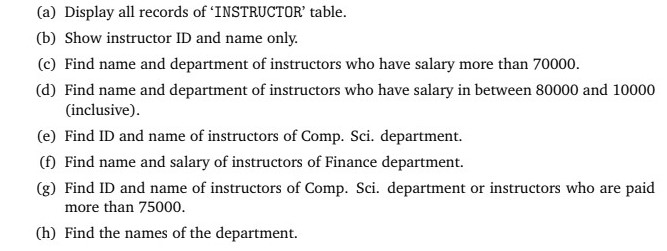
\includegraphics[width=\linewidth]{Screenshot 2022-09-03 220456.jpg}
\end{figure}\newline
\textbf{Analysis of the problem: }We can use SELECT command for the given queries to find or display anything inside our table\newline

\subsection*{(a)}
\textbf{\textit{\large Code:}}
\begin{minted}{SQL}
SELECT * FROM INSTRUCTOR;
\end{minted}

\subsection*{(b)}
\textbf{\textit{\large Code:}}
\begin{minted}{SQL}
SELECT ID, NAME FROM INSTRUCTOR;
\end{minted}

\subsection*{(c)}
\textbf{\textit{\large Code:}}
\begin{minted}{SQL}
SELECT NAME, DEPT_NAME FROM INSTRUCTOR WHERE SALARY > 70000;
\end{minted}

\subsection*{(d)}
\textbf{\textit{\large Code:}}
\begin{minted}{SQL}
SELECT NAME, DEPT_NAME FROM INSTRUCTOR WHERE SALARY > 10000 AND SALARY <80000;
\end{minted}

\subsection*{(e)}
\textbf{\textit{\large Code:}}
\begin{minted}{SQL}
SELECT ID, Name FROM INSTRUCTOR WHERE DEPT_NAME = 'Comp. Sci.';
\end{minted}

\subsection*{(f)}
\textbf{\textit{\large Code:}}
\begin{minted}{SQL}
SELECT NAME, SALARY FROM INSTRUCTOR WHERE DEPT_NAME = 'Finance';
\end{minted}

\subsection*{(g)}
\textbf{\textit{\large Code:}}
\begin{minted}{SQL}
SELECT ID, Name FROM INSTRUCTOR WHERE DEPT_NAME = 'Comp. Sci.' OR SALARY >75000;
\end{minted}

\subsection*{(h)}
\textbf{\textit{\large Code:}}
\begin{minted}{SQL}
SELECT DISTINCT(DEPT_NAME) FROM INSTRUCTOR;
\end{minted}

\textbf{Explanation of solution: }The SELECT command selects any information needed on the table that is specified using FROM command. WHERE command can determine which statements we are selecting and * command selects all records from any table.\\
\newline
\textbf{Findings: }We can select multiple attributes from each table and the statement after a WHERE command can work like a boolean expression.
\end{document}
